\documentclass[tikz]{standalone}
\usepackage{fourier}
\usepackage{tikz}

\begin{document}
  %:-+-+-+-+- Engendré par : http://math.et.info.free.fr/TikZ/TableauxVariations/
  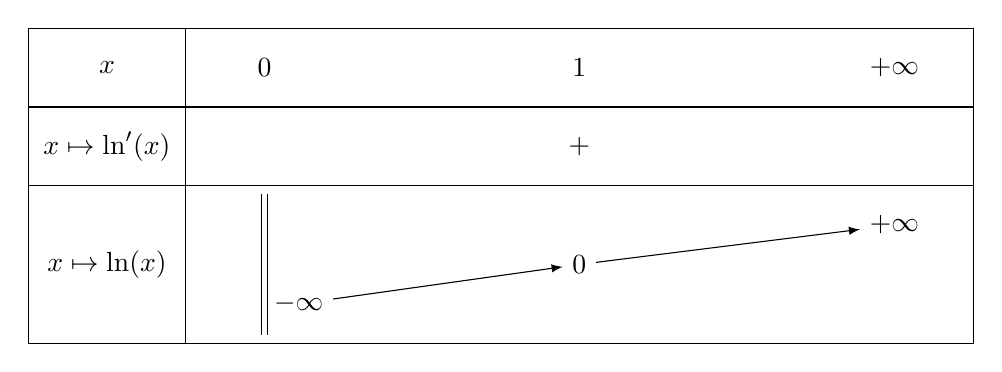
\begin{tikzpicture}[]
  	% Styles
  	\tikzstyle{cadre}=[thin]
  	\tikzstyle{fleche}=[->,>=latex,thin]
  	\tikzstyle{nondefini}=[lightgray]
  	% Dimensions Modifiables
  	\def\Lrg{2}
  	\def\HtX{1}
  	\def\HtY{0.5}
  	% Dimensions Calculées
  	\def\lignex{-0.5*\HtX}
  	\def\lignef{-1.5*\HtX}
  	\def\separateur{-0.5*\Lrg}
  	% Largeur du tableau
  	\def\gauche{-1.5*\Lrg}
  	\def\droite{4.5*\Lrg}
  	% Hauteur du tableau
  	\def\haut{0.5*\HtX}
  	\def\bas{-2.5*\HtX-2*\HtY}
  	\fill [white] (\gauche, \haut) rectangle (\droite,\bas);
  	% Ligne de l'abscisse : x
  	\node at (-1*\Lrg,0) {$x$};
  	\node at (0*\Lrg,0) {$0$};
  	\node at (2*\Lrg,0) {$1$};
  	\node at (4*\Lrg,0) {$+\infty$};
  	% Ligne de la dérivée : f'(x)
  	\node at (-1*\Lrg,-1*\HtX) {$x \mapsto \ln'(x)$};
  	\node at (0*\Lrg,-1*\HtX) {};
  	\node at (1*\Lrg,-1*\HtX) {};
  	\node at (2*\Lrg,-1*\HtX) {$+$};
  	\node at (3*\Lrg,-1*\HtX) {};
  	\node at (4*\Lrg,-1*\HtX) {};
  	% Ligne de la fonction : f(x)
  	\node  at (-1*\Lrg,{-2*\HtX+(-1)*\HtY}) {$x \mapsto \ln(x)$};
  	\node[left] (f1) at (0*\Lrg,{-2*\HtX+(0)*\HtY}) {};
  	\node[right] (f2) at (0*\Lrg,{-2*\HtX+(-2)*\HtY}) {$-\infty$};
  	\node (f3) at (2*\Lrg,{-2*\HtX+(-1)*\HtY}) {$0$};
  	\node (f4) at (4*\Lrg,{-2*\HtX+(0)*\HtY}) {$+\infty$};
  	% Flèches
  	\draw[fleche] (f2) -- (f3);
  	\draw[fleche] (f3) -- (f4);
  	% Doubles barres
  	\draw[double distance=2pt] (0*\Lrg,\lignef-0.1*\HtX) -- (0*\Lrg,\bas+0.1*\HtX);
  	% Encadrement
  	\draw[cadre] (\separateur,\haut) -- (\separateur,\bas);
  	\draw[cadre] (\gauche,\haut) rectangle  (\droite,\bas);
  	\draw[cadre] (\gauche,\lignex) -- (\droite,\lignex);
  	\draw[cadre] (\gauche,\lignef) -- (\droite,\lignef);
  \end{tikzpicture}
  %:-+-+-+-+- Fin
\end{document}
